\subsection[Minerology]{Minerology}
\begin{frame}
  \frametitle{Minerology (I)}

  A deep understanding of the nuclear fuel cycle requires study of
  ``exotic'' pentavalent uranium minerals that can form under specific
  mine or storage facility conditions.  One such mineral,
  {\ufivemineral}, has recently been synthesized.

  \qquad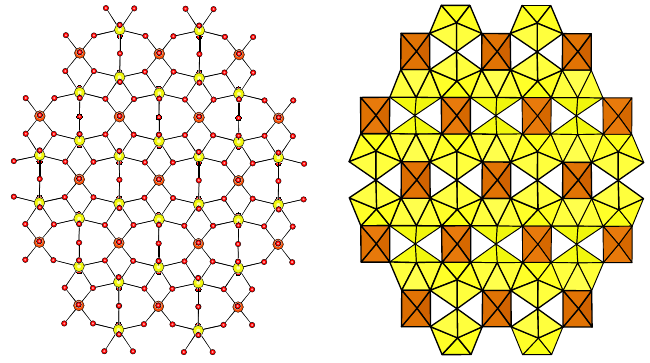
\includegraphics[width=0.7\linewidth]{xas/u5mineral.png}

  \begin{block}{}
    XRD is an indirect measure of valence | XAS is a direct measure!
  \end{block}

  \begin{bottomnote}[0.5][19]
    N. Belai et el., \textit{Pentavalent Uranium Oxide via Reduction
    of [UO$_2$]$^{2+}$ Under Hydrothermal Reaction Conditions},
    Inorg. Chem., 2008, 47 (21), pp 10135--10140,
    \doiref{10.1021/ic801534m}[LightBlue4]
  \end{bottomnote}
\end{frame}
\begin{frame}
  \frametitle{Minerology (II)}
  XAS on \ufivemineral

  \begin{columns}[T]
    \begin{column}{0.5\linewidth}
      \begin{center}
        \small
        XANES data\\
        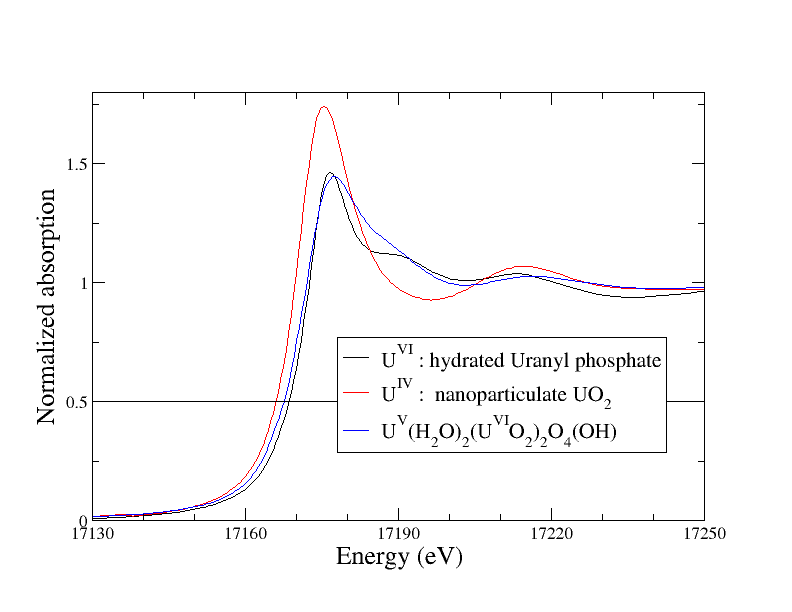
\includegraphics[width=\linewidth]{xas/u5norm.png}\\
        We see evidence of U$^{\mathrm{V}}$ by  the intermediate edge position
        between our U$^{\mathrm{IV}}$ and U$^{\mathrm{VI}}$ standards.
      \end{center}
    \end{column}
    \begin{column}{0.5\linewidth}
      \begin{center}
        \small
        EXAFS analysis\\
        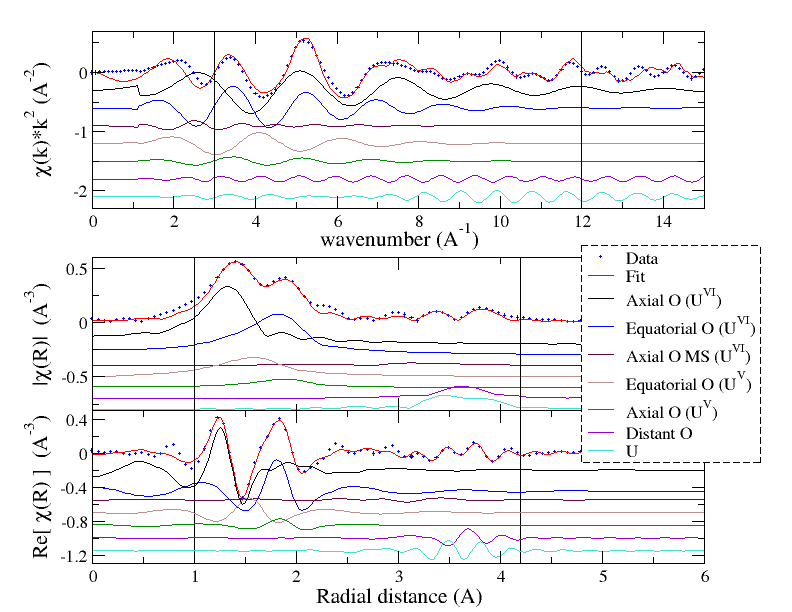
\includegraphics[width=\linewidth]{xas/u5chikr.png}\\
        The crystal structure refined from the XRD is consistent with
        the EXAFS data.
      \end{center}
    \end{column}
  \end{columns}

%   \bigskip

%   The data on this page has been redacted as the paper has not yet
%   been published.  The data that were here demonstrated that the
%   mineral contains U$^{\mathrm{V}}$ and that the structure refined
%   from XRD is consistent with the EXAFS data.

  \begin{bottomnote}[0.5][19]
    N. Belai et el., \textit{Pentavalent Uranium Oxide via Reduction
    of [UO$_2$]$^{2+}$ Under Hydrothermal Reaction Conditions},
    Inorg. Chem., 2008, 47 (21), pp 10135--10140,
    \doiref{10.1021/ic801534m}[LightBlue4]
  \end{bottomnote}
\end{frame}


